%% derived from https://tex.stackexchange.com/questions/357538/graph-of-a-parabola-on-pgfplots
%% Thanks to Stefan Pinnow
%%     https://tex.stackexchange.com/users/95441/stefan-pinnow

\begin{figure}
\centering
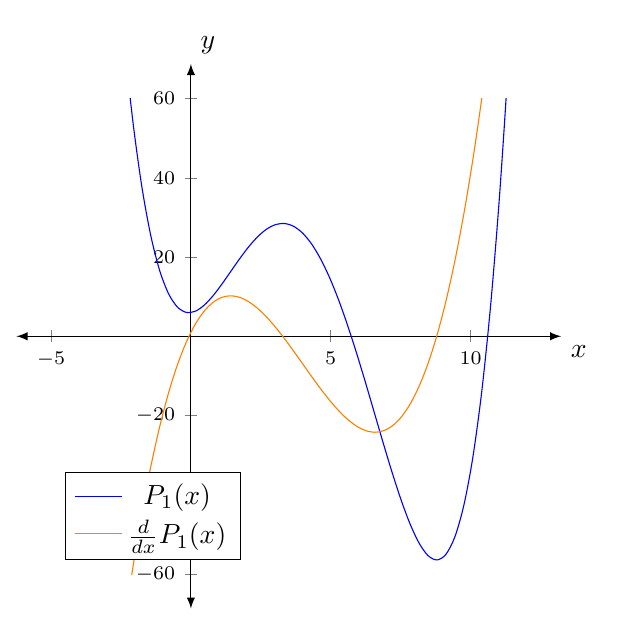
\begin{tikzpicture}
    \begin{axis}[
        width=3in,
        height=3in,
        axis lines=middle,
        xmin=-5,
        xmax=12,
        ymin=-60,
        ymax=60,
%        xtick={20000},
        % ---------------------------------------------------------------------
        % you don't want the ticks/tick labels to be scaled
        scaled ticks=false,
%        % and the tick labels are shown by default the way you want them,
%        % so you don't need to specify them explicitely
%        xticklabels={$20000$},
        % ---------------------------------------------------------------------
 %       ytick={\empty},
        legend pos=south west,
        ticklabel style={font=\scriptsize},
        xlabel=$x$,
        ylabel=$y$,
        axis line style={
            latex-latex,
            shorten >=-12.5pt,
            shorten <=-12.5pt,
        },
        xlabel style={at={(ticklabel* cs:1)}, xshift=12.5pt, anchor=north west},
        ylabel style={at={(ticklabel* cs:1)}, yshift=12.5pt, anchor=south west},
    ]

        \addplot[samples=51,smooth,domain=-4:12,color=blue] {0.125 * x^4 -2* x^3 + 7 * x^2 + x + 6};
        \addlegendentry{\(P_1(x)\)}
        \addplot[samples=51,smooth,domain=-4:12,color=orange] {0.5 * x^3 -6* x^2 + 14 * x + 1};
        \addlegendentry{\(\frac{d}{dx}P_1(x)\)}

    \end{axis}


\end{tikzpicture}
%
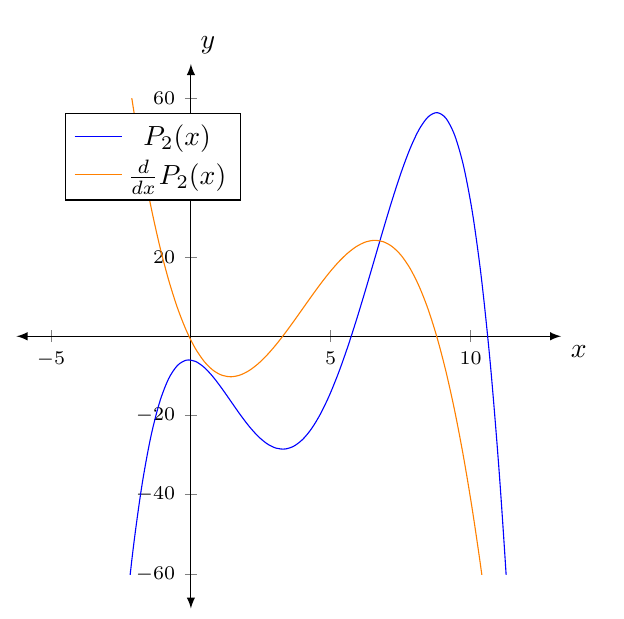
\begin{tikzpicture}
    \begin{axis}[
        width=3in,
        height=3in,
        axis lines=middle,
        xmin=-5,
        xmax=12,
        ymin=-60,
        ymax=60,
%        xtick={20000},
        % ---------------------------------------------------------------------
        % you don't want the ticks/tick labels to be scaled
        scaled ticks=false,
%        % and the tick labels are shown by default the way you want them,
%        % so you don't need to specify them explicitely
%        xticklabels={$20000$},
        % ---------------------------------------------------------------------
 %       ytick={\empty},
        legend pos=north west,
        ticklabel style={font=\scriptsize},
        xlabel=$x$,
        ylabel=$y$,
        axis line style={
            latex-latex,
            shorten >=-12.5pt,
            shorten <=-12.5pt,
        },
        xlabel style={at={(ticklabel* cs:1)}, xshift=12.5pt, anchor=north west},
        ylabel style={at={(ticklabel* cs:1)}, yshift=12.5pt, anchor=south west},
    ]

        \addplot[samples=51,smooth,domain=-4:12,color=blue] {-0.125 * x^4 +2* x^3 - 7 * x^2 - x - 6};
        \addlegendentry{\(P_2(x)\)}
        \addplot[samples=51,smooth,domain=-4:12,color=orange] {-0.5 * x^3 +6* x^2 - 14 * x - 1};
        \addlegendentry{\(\frac{d}{dx}P_2(x)\)}
    \end{axis}


\end{tikzpicture}
\caption{Quartics $P_1(x)$ and $P_2(x)$ from Figure~\ref{fig.quartic} and their derivatives.
\textcolor{blue}{In blue ${y=P_1(x)}$ and ${y=P_2(x)}$}.
\textcolor{orange}{In orange ${y=-\frac{d}{dx} P_1(x)}$ and ${y=-\frac{d}{dx} P_2(x)}$}}
\label{fig.quartic.deriv}
\end{figure}
